\section{Wprowadzenie}
Niniejszy tekst stanowi dokumentację techniczną opisującą szczegóły architektoniczne i implementacyjne systemu projektowanego w ramach pracy inżynierskiej.

Tematem projektu jest stworzenie systemu przechowującego i udostępniającego pliki w rozproszonej infrastrukturze. System można uruchomić na zespole heterogenicznych węzłów tworzących klaster. Wszystkie informacje o akcjach podejmowanych przez użytkowników są gromadzone, a na ich podstawie użytkownicy zostają dopasowani do różnych klas odpowiadających ich wymaganiom.

\subsection{Opis problemu}
Współcześnie bardzo wzrosło zapotrzebowanie na usługi przechowywania plików. Na rynku istnieje kilka rozwiązań pozwalających na przechowywanie plików. Są to między innymi Amazon S3, Riak Cloud Storage czy Ceph.

Celem projektu był stworzenie o podobnej funkcjonalności, pozwalającej użytkownikom tworzyć, czytać, zapisywać i usuwać pliki. Użytkownicy nie muszą znać dokładnego miejsca fizycznego położenia swoich danych. System powinien tak lokować pliki w poszczególnych magazynach danych (storage), aby zasoby systemowe były równomiernie i efektywnie wykorzystane.

\subsection{Opis produktu}
Dostarczony produkt to rozproszona aplikacja Erlang/OTP. Każdy magazyn (storage) to samodzielna instancja komunikująca się z pozostałymi magazynami. System przeznaczony jest do uruchomienia na klastrze złożonym z kilku - kilkunastu maszyn (węzłów) połączonych w sieć lokalną LAN. Możliwa jest również komunikacja poprzez sieć Internet.

Użytkownik może wykonywać operacje CRUD (Create, Read, Update, Delete) na swoich plikach korzystając z trzech interfejsów:
\begin{itemize}
	\item biblioteki klienckiej (napisanej w Erlangu)
	\item RESTful API dostępnego każdym węźle przez protokół HTTP
	\item manualnie, korzystając z udostępnionego w przeglądarce GUI
\end{itemize}

Własne pliki można udostępniać innym użytkownikom w trybie tylko do odczytu.

Aplikacja monitoruje wszystkie akcje, jakie podejmują użytkownicy. Są one zapisywane w bazie danych (aktualnie jest to SQLite 3). Przy ich pomocy system ustala priorytety dla poszczególnych zapytań podczas fazy schedulingu.

W razie potrzeby do systemu można dodać nowy węzeł. Nie zakłóca to jego pracy i nie wymaga zatrzymywania systemu. W przypadku wyłączenia jednego z węzłów system nadal funkcjonuje poprawnie a dane z odłączonego węzła są niedostępne do czasu jego ponownego podłączenia.

\subsection{Wymagania funkcjonalne}
Wymagania funkcjonalne zostały zebrane w postaci diagramu przypadków użycia przedstawionego na \autoref{fig:use-case}. W systemie występuje tylko jeden typ użytkownika, którego akcje są bezpośrednio obsługiwane przez system. Jest to użytkownik końcowy, który ma możliwość wykonywania podstawowych operacji na plikach.

Innym typem użytkownika jest administrator. System nie oferuje jednak funkcjonalności przydatnej w pracy administratora. Konfiguracja dobywa się poprzez pliki konfiguracyjne a za zarządzanie węzłem odpowiada mechanizm supervisorów.

\begin{figure}[!htbp]
	\centering
	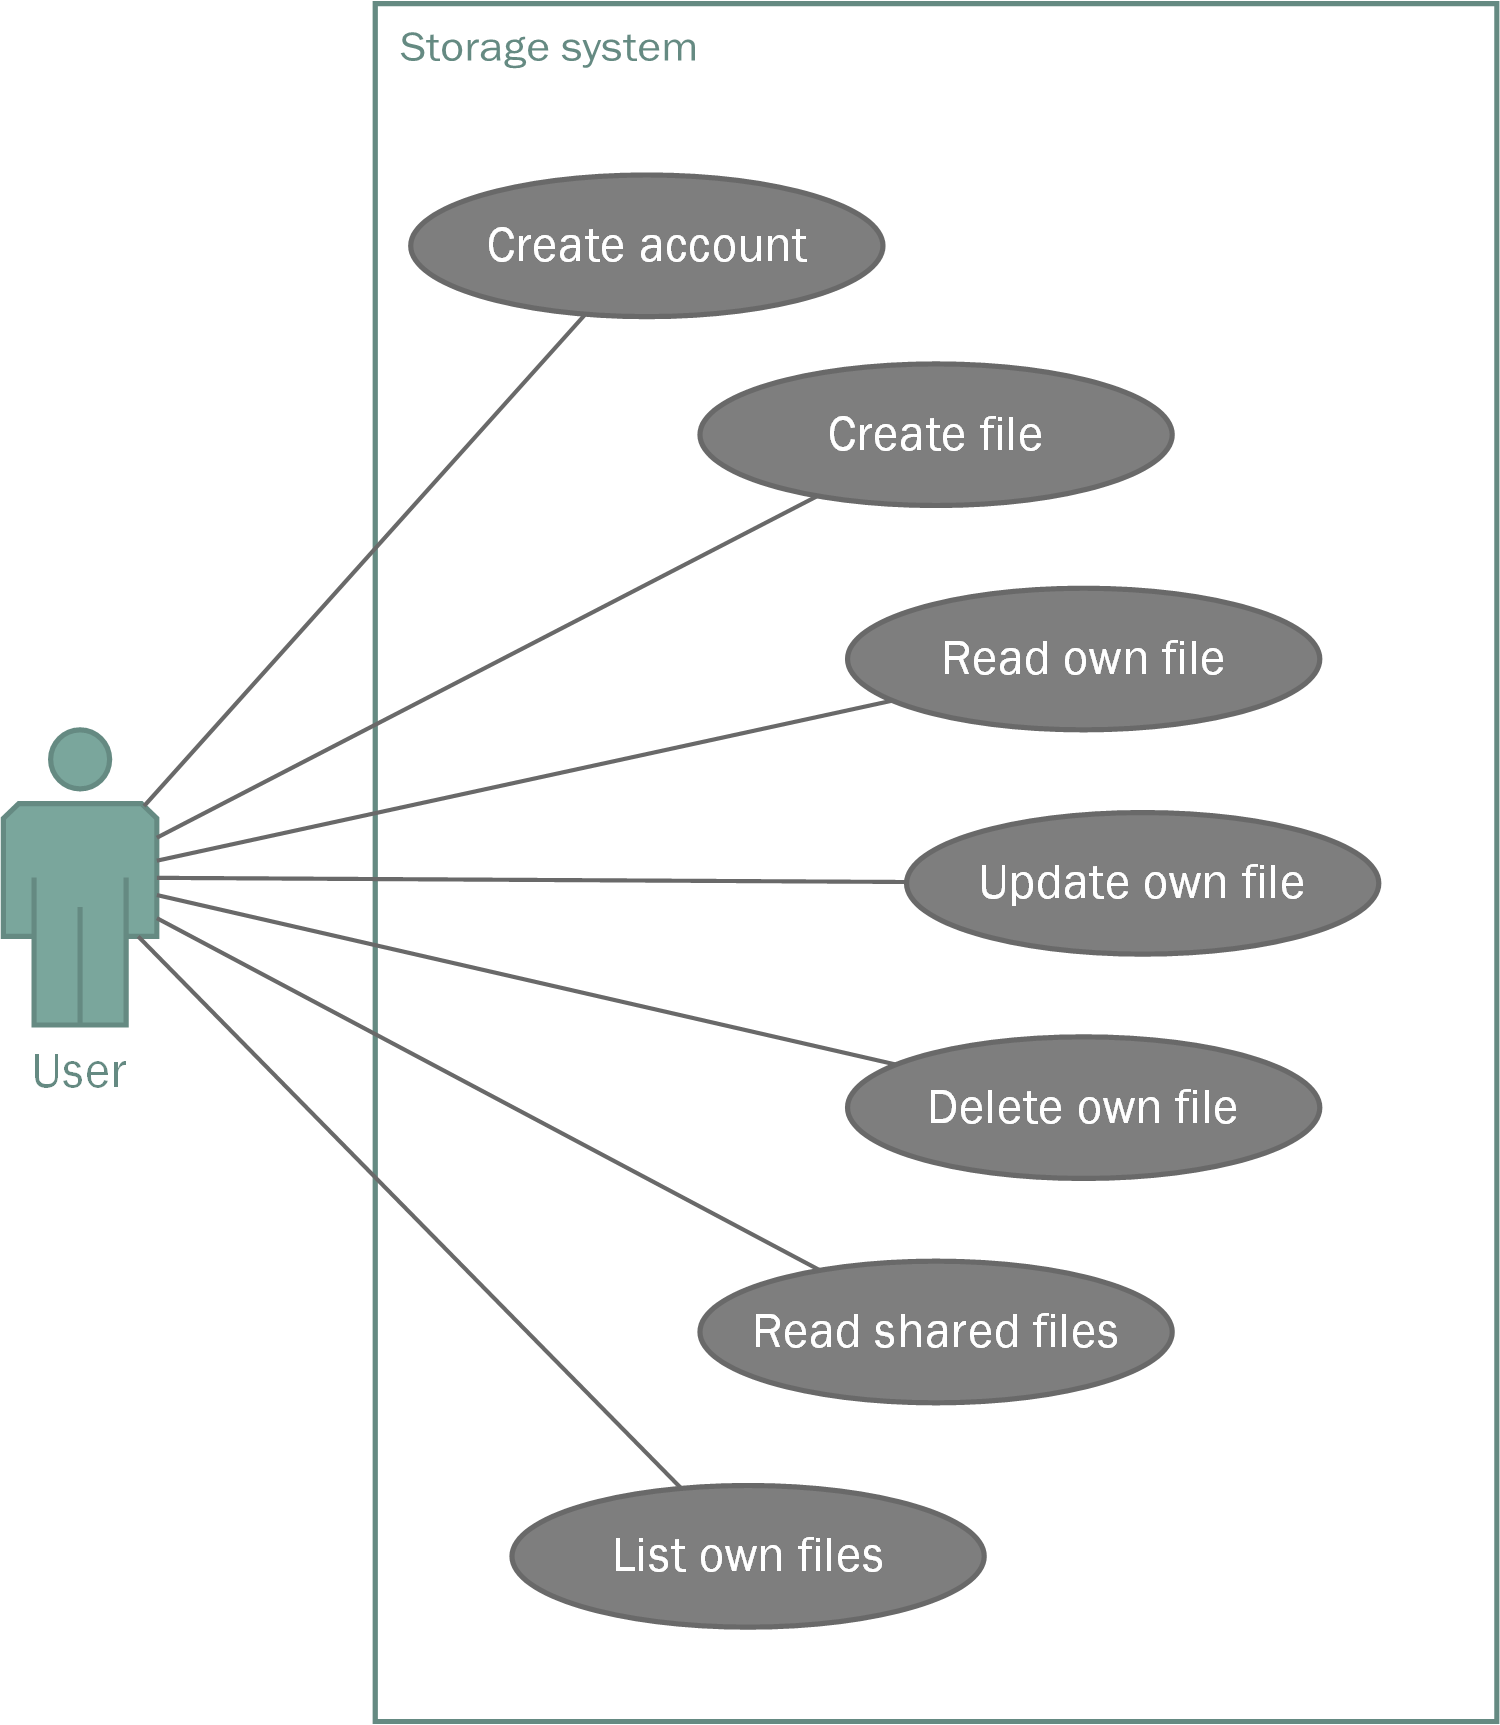
\includegraphics[width=0.8\textwidth]{use-case}
	\caption[Diagram przypadków użycia użytkownika systemu.]{Diagram przypadków użycia użytkownika systemu. Oprócz podstawowych operacji CRUD użytkownik może wylistować własne pliki i założyć konto w systemie.}
	\label{fig:use-case}
\end{figure}

\subsection{Inne wymagania}
Pozostałe wymagania dotyczą nie funkcjonalności systemu, a jego pożądanych cech:
\begin{itemize}
	\item system zdecentralizowany
	\item rozwiązanie wieloplatformowe
	\item system powinien gromadzić informacje o akcjach użytkowników
	\item zachowanie użytkownika powinno mieć wpływ na priorytet jego zapytań
\end{itemize}
